\documentclass[12pt]{article}
\usepackage{geometry}
\usepackage{graphicx}
\renewcommand{\familydefault}{\sfdefault}
\usepackage{helvet}
\title{PHC 6000: Homework 1}
\author{Joe Brew}
\usepackage{Sweave}
\begin{document}
\newgeometry{margin=1.5cm}
\Sconcordance{concordance:homework1.tex:homework1.Rnw:%
1 7 1 1 0 45 1 1 116 1 3 17 0 1 2 9 1 1 59 1 3 21 0 1 2 1 4 1 2 10 1 1 %
2 4 0 1 2 6 1 1 2 1 0 4 1 3 0 1 2 8 1 1 2 1 0 4 1 1 2 3 0 1 2 8 1 1 2 1 %
0 3 1 1 2 1 0 2 1 1 12 11 0 1 3 8 1 1 5 3 0 1 3 1 0 1 1 1 2 1 0 1 2 1 0 %
1 2 1 0 1 3 1 0 1 4 3 0 1 4 3 0 1 4 3 0 1 4 3 0 1 3 1 0 1 4 3 0 1 4 3 0 %
1 4 3 0 1 4 3 0 1 3 1 0 1 1 1 2 1 0 1 2 1 0 1 2 1 0 1 3 1 0 1 1 1 3 1 0 %
1 1 1 3 1 0 1 1 1 3 2 0 1 3 4 0 1 2 2 1}

\maketitle
\begin{center}
UF-ID: 0402-8902
\end{center}

\vspace{30mm}
\tableofcontents

\newpage
\section*{Problem 1: Incidence versus Prevalence}
\addcontentsline{toc}{section}{Problem 1: Incidenve versus Prevalence}

\subsection*{A}
Point prevalence.

\subsection*{B}
Since we dont have exact information on each person \textbf{incidence rate} best describes this fraction.  Incidence rate addresses the fact that we don't have specific information on all population members and the fact that there is a time element (cases per person-time units). 

\subsection*{C}
Assuming that the "numer of cervical cancer cases in Florida in 2009" refers both to those which were prevalent at the beginning of the year as well as incident 2009 cases, then the correct answer is \textbf{period prevalence}.

\section*{Problem 2: Survival analysis assumptions}
\addcontentsline{toc}{section}{Problem 2: Survival analysis assumptions}
\subsection*{Differences}
\addcontentsline{toc}{subsection}{Differences}
Two differences between the actuarial / life table approach and the Kaplan-Meier method are: 
\begin{enumerate}
\item The actuarial / life table method requires a priori knowledge of time intervals to be used (the Kaplan-Meier method creates intervals as a function of actual event/censorship times).
\item In the actuarial / life table method (unlike Kaplan-Meier), it is not necessary to know the exact time of event or censorship.  \\
\end{enumerate}

\subsection*{Shared assumptions}
\addcontentsline{toc}{subsection}{Shared assumptions}
Both the actuarial / life table method as well as the Kaplan-Meier method assume that : 
\begin{enumerate}
\item There are no secular trends (ie, big changes from outside influences).
\item The censored population are no different (in terms of probability of having event) from the non-censored population (ie, independence of event and censoring.) \\
\end{enumerate}

\newpage
\section*{Problem 3: Cumulative incidence}
\addcontentsline{toc}{section}{Problem 3: Cumulative incidence}


% latex table generated in R 3.0.2 by xtable 1.7-1 package
% Mon Jan 20 16:57:50 2014
\begin{table}[ht]
\centering
\caption{Life Table} 
{\tiny
\begin{tabular}{rlrrrrrrrr}
  \hline
 & interval & casesAtStart & deathsDuring & withdrawsDuring & casesAtRisk & condProbOfEvent & condProbOfSurv & cumProbOfSurv & cumProbOfEvent \\ 
  \hline
1 & 0-5 & 0.00 & 2.00 & 1.00 & 10.00 & 0.20 & 0.80 & 0.80 & 0.20 \\ 
  2 & 6-10 & 3.00 & 2.00 & 1.00 & 7.00 & 0.29 & 0.71 & 0.57 & 0.43 \\ 
  3 & 11-15 & 6.00 & 3.00 & 0.00 & 4.00 & 0.75 & 0.25 & 0.18 & 0.82 \\ 
  4 & 16-20 & 9.00 & 1.00 & 0.00 & 1.00 & 1.00 & 0.00 & 0.00 & 1.00 \\ 
   \hline
\end{tabular}
}
\end{table}
[1] "% latex table generated in R 3.0.2 by xtable 1.7-1 package\n% Mon Jan 20 16:57:50 2014\n\\begin{table}[ht]\n\\centering\n\\caption{Life Table} \n{\\tiny\n\\begin{tabular}{rlrrrrrrrr}\n  \\hline\n & interval & casesAtStart & deathsDuring & withdrawsDuring & casesAtRisk & condProbOfEvent & condProbOfSurv & cumProbOfSurv & cumProbOfEvent \\\\ \n  \\hline\n1 & 0-5 & 0.00 & 2.00 & 1.00 & 10.00 & 0.20 & 0.80 & 0.80 & 0.20 \\\\ \n  2 & 6-10 & 3.00 & 2.00 & 1.00 & 7.00 & 0.29 & 0.71 & 0.57 & 0.43 \\\\ \n  3 & 11-15 & 6.00 & 3.00 & 0.00 & 4.00 & 0.75 & 0.25 & 0.18 & 0.82 \\\\ \n  4 & 16-20 & 9.00 & 1.00 & 0.00 & 1.00 & 1.00 & 0.00 & 0.00 & 1.00 \\\\ \n   \\hline\n\\end{tabular}\n}\n\\end{table}\n"
\subsection*{1}
The cumulative probability of death over the 20 months period using the life table interval approach is 1. \\

\subsection*{2}
The cumulative probability of survival over the 20 months period using the life table interval approach is 0. \\

\subsection*{3}
The Kaplan-Meier approach, unlike the Life Table approach, relies on setting up time intervals as a function of the actual time of event / withdrawal.  See below table:


% latex table generated in R 3.0.2 by xtable 1.7-1 package
% Mon Jan 20 16:57:50 2014
\begin{table}[ht]
\centering
\caption{Kaplan-Meier Table} 
{\tiny
\begin{tabular}{rrrrrrrrrr}
  \hline
 & interval & casesAtStart & deathsDuring & withdrawsDuring & casesAtRisk & condProbOfEvent & condProbOfSurv & cumProbOfSurv & cumProbOfEvent \\ 
  \hline
1 & 3.00 & 0.00 & 1.00 & 0.00 & 10.00 & 0.10 & 0.90 & 0.90 & 0.10 \\ 
  2 & 4.00 & 1.00 & 0.00 & 1.00 & 9.00 & 0.00 & 1.00 & 0.90 & 0.10 \\ 
  3 & 7.00 & 3.00 & 1.00 & 0.00 & 7.00 & 0.14 & 0.86 & 0.86 & 0.14 \\ 
  4 & 8.00 & 4.00 & 0.00 & 1.00 & 6.00 & 0.00 & 1.00 & 0.86 & 0.14 \\ 
  5 & 10.00 & 5.00 & 1.00 & 0.00 & 5.00 & 0.20 & 0.80 & 0.80 & 0.20 \\ 
  6 & 13.00 & 7.00 & 1.00 & 0.00 & 3.00 & 0.33 & 0.67 & 0.53 & 0.47 \\ 
  7 & 15.00 & 8.00 & 1.00 & 0.00 & 2.00 & 0.50 & 0.50 & 0.33 & 0.67 \\ 
  8 & 20.00 & 9.00 & 1.00 & 0.00 & 1.00 & 1.00 & 0.00 & 0.00 & 1.00 \\ 
   \hline
\end{tabular}
}
\end{table}
[1] "% latex table generated in R 3.0.2 by xtable 1.7-1 package\n% Mon Jan 20 16:57:50 2014\n\\begin{table}[ht]\n\\centering\n\\caption{Kaplan-Meier Table} \n{\\tiny\n\\begin{tabular}{rrrrrrrrrr}\n  \\hline\n & interval & casesAtStart & deathsDuring & withdrawsDuring & casesAtRisk & condProbOfEvent & condProbOfSurv & cumProbOfSurv & cumProbOfEvent \\\\ \n  \\hline\n1 & 3.00 & 0.00 & 1.00 & 0.00 & 10.00 & 0.10 & 0.90 & 0.90 & 0.10 \\\\ \n  2 & 4.00 & 1.00 & 0.00 & 1.00 & 9.00 & 0.00 & 1.00 & 0.90 & 0.10 \\\\ \n  3 & 7.00 & 3.00 & 1.00 & 0.00 & 7.00 & 0.14 & 0.86 & 0.86 & 0.14 \\\\ \n  4 & 8.00 & 4.00 & 0.00 & 1.00 & 6.00 & 0.00 & 1.00 & 0.86 & 0.14 \\\\ \n  5 & 10.00 & 5.00 & 1.00 & 0.00 & 5.00 & 0.20 & 0.80 & 0.80 & 0.20 \\\\ \n  6 & 13.00 & 7.00 & 1.00 & 0.00 & 3.00 & 0.33 & 0.67 & 0.53 & 0.47 \\\\ \n  7 & 15.00 & 8.00 & 1.00 & 0.00 & 2.00 & 0.50 & 0.50 & 0.33 & 0.67 \\\\ \n  8 & 20.00 & 9.00 & 1.00 & 0.00 & 1.00 & 1.00 & 0.00 & 0.00 & 1.00 \\\\ \n   \\hline\n\\end{tabular}\n}\n\\end{table}\n"\begin{center}
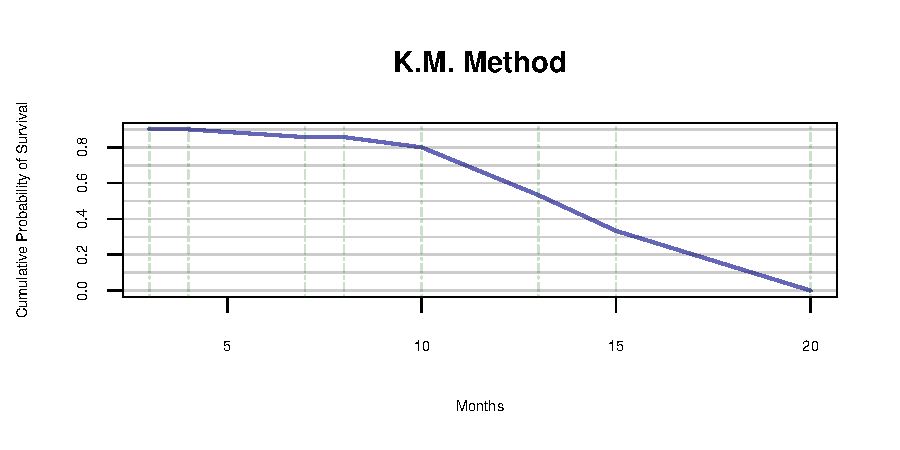
\includegraphics{homework1-005}
\end{center}

\newpage
\section*{Problem 4: Incidence density - individual data}
\addcontentsline{toc}{section}{Problem 4: Incidence density - individual data}

\subsection*{Total number of person-years}
\addcontentsline{toc}{subsection}{Total number of person-years}

The total number of person-years contributed is equal to the sum of each participants' time before censoring or onset of disease.

\begin{Schunk}
\begin{Sinput}
> answer <- 3 + 5 + 2.4 + 3.6 + 4 + 1.9 + 4.1 + 2 + 3 + 5
\end{Sinput}
\end{Schunk}
Answer: \textbf{34 person-years}

\subsection*{5-year incidence density}
\addcontentsline{toc}{subsection}{5-year incidence density}

The incidence density is a fraction which contains the number of incident cases in (numerator) over the sum of the person-time of all individuals at risk (denominator).  

\begin{Schunk}
\begin{Sinput}
> personNum <- 1:10
> status <- c("d", "c", "c", "d", "c", "c", "c", "d", "c", "c")
> interval <- c(3,5,2.4,3.6,4,1.9,4.1,2,3,5)
> prob4 <- as.data.frame(cbind(personNum, status, interval))
> answer <- nrow(prob4[which(prob4$status=="d"),]) / sum(interval)
\end{Sinput}
\end{Schunk}


In this case it is equal to \textbf{0.088} new cases per person-year (work shown above).

\section*{Problem 5: Incidence rate - group data}
\addcontentsline{toc}{section}{Problem 5: Incidence rate - group data}

Using the midpoint estimation method to calculate the incidence rate of X assumes a normal distribution of removal from study population time (either by censoring or event).  This assumption allows for us to simply take the (initial population plus the end population) divided by two.  Once the midpoint population has been estimated, the incidence rate is simply the number of incident cases over the midpoint population (for a given set of time - in this case, two years):

\begin{Schunk}
\begin{Sinput}
> initialPop <- 300
> newCases <- 5
> censored <- 35
> endPop <- initialPop - newCases - censored
> midPointPop <- (initialPop + endPop) / 2 
> incidenceRate <- newCases / midPointPop
\end{Sinput}
\end{Schunk}

\textbf{0.018} incident cases for every 2 person-years (equivalent to 0.009 per person-year).

\newpage
\section*{Details}
\addcontentsline{toc}{section}{Details}
\subsection*{Problem 3 (work shown)}
\addcontentsline{toc}{subsection}{Problem 3 (work shown)}
\begin{tiny}
\begin{Schunk}
\begin{Sinput}
> library(xtable)
> personNum <- as.numeric(c(1:10))
> months <- as.numeric(as.character(c(10, 12, 4, 3, 7, 5, 8, 15, 13, 20)))
> status <- c("d", "d", "c", "d", "d", "d", "c", "d", "d", "d")
> prob3 <- as.data.frame(cbind(personNum, months, status),
+                        stringsAsFactors = FALSE)
> prob3$months <- as.numeric(as.character(prob3$months))
> prob3$personNum <- as.numeric(as.character(prob3$personNum))
> prob3$interval <- ifelse(prob3$months <= 5,
+                          "0-5",
+                          ifelse(prob3$months >=6 &
+                                   prob3$months <=10,
+                                 "6-10", 
+                                 ifelse(prob3$months >=11 &
+                                          prob3$months <=15,
+                                        "11-15",
+                                        ifelse(prob3$months >=16 &
+                                                 prob3$months <=20,
+                                               "16-20",
+                                               NA))))
> interval <- c("0-5", "6-10", "11-15", "16-20")
> casesAtStart <- c(NA, NA, NA, NA)
> deathsDuring <- c(NA, NA, NA, NA)
> withdrawsDuring <- c(NA, NA, NA, NA)
> casesAtRisk <- c(NA, NA, NA, NA)
> condProbOfEvent <- c(NA, NA, NA, NA)
> condProbOfSurv <- c(NA, NA, NA, NA)
> cumProbOfSurv <- c(NA, NA, NA, NA)
> cumProbOfEvent <- c(NA, NA, NA, NA)
> lifeTable <- as.data.frame(cbind(interval, casesAtStart, deathsDuring,
+                                  withdrawsDuring, casesAtRisk,
+                                  condProbOfEvent, condProbOfSurv,
+                                  cumProbOfSurv, cumProbOfEvent))
> #casesAtStart
> lifeTable$casesAtStart <- as.numeric(lifeTable$casesAtStart)
> lifeTable$casesAtStart[which(lifeTable$interval== "0-5")] <- 0
> lifeTable$casesAtStart[which(lifeTable$interval== "6-10")] <- 
+   nrow(prob3[which(prob3$months <= 5),])
> lifeTable$casesAtStart[which(lifeTable$interval== "11-15")] <- 
+   nrow(prob3[which(prob3$months <= 10),])
> lifeTable$casesAtStart[which(lifeTable$interval== "16-20")] <- 
+   nrow(prob3[which(prob3$months <= 15),])
> #deathsDuring
> lifeTable$deathsDuring <- as.numeric(lifeTable$deathsDuring)
> lifeTable$deathsDuring[which(lifeTable$interval == "0-5")] <- 
+   nrow(prob3[which(prob3$status=="d" 
+                    & prob3$months >=0
+                    & prob3$months <=5),])
> lifeTable$deathsDuring[which(lifeTable$interval == "6-10")] <- 
+   nrow(prob3[which(prob3$status=="d" 
+                    & prob3$months >=6
+                    & prob3$months <=10),])
> lifeTable$deathsDuring[which(lifeTable$interval == "11-15")] <- 
+   nrow(prob3[which(prob3$status=="d" 
+                    & prob3$months >=11
+                    & prob3$months <=15),])
> lifeTable$deathsDuring[which(lifeTable$interval == "16-20")] <- 
+   nrow(prob3[which(prob3$status=="d" 
+                    & prob3$months >=16
+                    & prob3$months <=20),])
> #withdrawsDuring
> lifeTable$withdrawsDuring <- as.numeric(lifeTable$withdrawsDuring)
> lifeTable$withdrawsDuring[which(lifeTable$interval == "0-5")] <- 
+   nrow(prob3[which(prob3$status=="c" 
+                    & prob3$months >=0
+                    & prob3$months <=5),])
> lifeTable$withdrawsDuring[which(lifeTable$interval == "6-10")] <- 
+   nrow(prob3[which(prob3$status=="c" 
+                    & prob3$months >=6
+                    & prob3$months <=10),])
> lifeTable$withdrawsDuring[which(lifeTable$interval == "11-15")] <- 
+   nrow(prob3[which(prob3$status=="c" 
+                    & prob3$months >=11
+                    & prob3$months <=15),])
> lifeTable$withdrawsDuring[which(lifeTable$interval == "16-20")] <- 
+   nrow(prob3[which(prob3$status=="c" 
+                    & prob3$months >=16
+                    & prob3$months <=20),])
> #casesAtRisk
> lifeTable$casesAtRisk <- as.numeric(lifeTable$casesAtRisk)
> lifeTable$casesAtRisk[which(lifeTable$interval== "0-5")] <- 10
> lifeTable$casesAtRisk[which(lifeTable$interval== "6-10")] <- 
+   nrow(prob3) - nrow(prob3[which(prob3$months <= 5),])
> lifeTable$casesAtRisk[which(lifeTable$interval== "11-15")] <- 
+   nrow(prob3) - nrow(prob3[which(prob3$months <= 10),])
> lifeTable$casesAtRisk[which(lifeTable$interval== "16-20")] <- 
+   nrow(prob3) - nrow(prob3[which(prob3$months <= 15),])
> #condProbOfEvent
> lifeTable$condProbOfEvent <- as.numeric(lifeTable$condProbOfEvent)
> lifeTable$condProbOfEvent <- lifeTable$deathsDuring / lifeTable$casesAtRisk
> #condProbOfSurv
> lifeTable$condProbOfSurv <- as.numeric(lifeTable$condProbOfSurv)
> lifeTable$condProbOfSurv <- 1- lifeTable$condProbOfEvent
> #cumProbOfSurv
> lifeTable$cumProbOfSurv <- as.numeric(lifeTable$cumProbOfSurv)
> lifeTable$cumProbOfSurv[1] <- lifeTable$condProbOfSurv[1]
> for (i in 2:4){
+   lifeTable$cumProbOfSurv[i] <-
+     lifeTable$condProbOfSurv[i]*lifeTable$condProbOfSurv[i-1]}
> #cumProbOfEvent
> lifeTable$cumProbOfEvent <- 1-lifeTable$cumProbOfSurv
\end{Sinput}
\end{Schunk}
\end{tiny}

\end{document}
